\documentclass[10pt]{article}
\usepackage[polish]{babel}
\usepackage[utf8]{inputenc}
\usepackage[T1]{fontenc}
\usepackage{amsmath}
\usepackage{amsfonts}
\usepackage{amssymb}
\usepackage[version=4]{mhchem}
\usepackage{stmaryrd}
\usepackage{graphicx}
\usepackage[export]{adjustbox}
\graphicspath{ {./images/} }
\usepackage{bbold}

\title{LIGA MATEMATYCZNA im. Zdzisława Matuskiego STYCZEŃ 2019 SZKOŁA PONADPODSTAWOWA }

\author{}
\date{}


\begin{document}
\maketitle
\section*{ZADANIE 1.}
Boki trójkąta \(A B C\) podzielono takimi punktami \(D, E, F, \dot{z}\) e \(\frac{|A D|}{|D B|}=\frac{|B E|}{|E C|}=\frac{|C F|}{|F A|}=6\). Wyznacz stosunek pola trójkąta \(D E F\) do pola trójkąta \(A B C\).\\
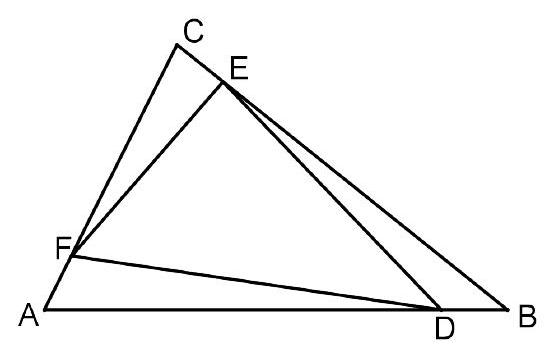
\includegraphics[max width=\textwidth, center]{2024_11_21_760b739d4da8f464884cg-1}

ZADANIE 2. Liczba dodatnia \(x\) jest \(p\) razy większa od liczby \(y\). Suma liczb \(x\) i \(y\) jest \(q\) razy większa od ich różnicy. Znajdź sumę \(p+q\) wiedząc, że \(p\) i \(q\) są liczbami całkowitymi dodatnimi.

\section*{ZADANIE 3.}
Wyznacz największą liczbę pięciocyfrową spełniającą warunki:

\begin{itemize}
  \item żadna cyfra nie jest zerem;
  \item pierwsze trzy cyfry tworzą liczbę, która jest 9 razy większa od liczby utworzonej przez dwie ostanie cyfry;
  \item trzy ostatnie cyfry tworzą liczbę, która jest 7 razy większa od liczby utworzonej przez pierwsze dwie cyfry.\\
(Uwaga. Przyjmujemy, że ostatnią cyfrą liczby jest cyfra jedności.)
\end{itemize}

\section*{ZADANIE 4.}
Wyznacz wszystkie liczby pierwsze \(p\) takie, że \(p+6, p+12, p+18, p+24\) są również liczbami pierwszymi.

\section*{ZADANIE 5.}
Znajdź wszystkie funkcje \(f: \mathbb{R} \backslash\{0,1\} \rightarrow \mathbb{R}\) spełniające warunek

\[
(1-x) f(x)-2 x f(1-x)=1
\]

dla każdej liczby rzeczywistej \(x\) różnej od 0 i 1.


\end{document}